\chapter{The Effect of Linked Selection}

When a beneficial allele arises as via a single mutation, it arises on
a particular genetic background, i.e. a particular haplotype (Figure \ref{fig:HIV_sweep}A). Imagine this mutation arising a region with no recombination, or in an
organism where genetic exchange is rare. If our beneficial allele
becomes established in the population, i.e. escapes loss by genetic
drift in those first few generation, it will start to increase in
frequency rapidly. As it does so, so will the alleles that happened to
be present on the haplotype that the mutation arose on (if those
other alleles are neutral or at least not too deleterious). These
other alleles are getting to hitchhiking along. The alleles that are
not on that background are swept out the population, so the net effect
of this selective sweep is to remove genetic diversity from the
population. Diversity will eventually recover as new mutations will
arise and some will slowly drift up in frequency. But in the
short-term selective sweeps remove genetic variation from
populations. 

\begin{figure}
\begin{center}
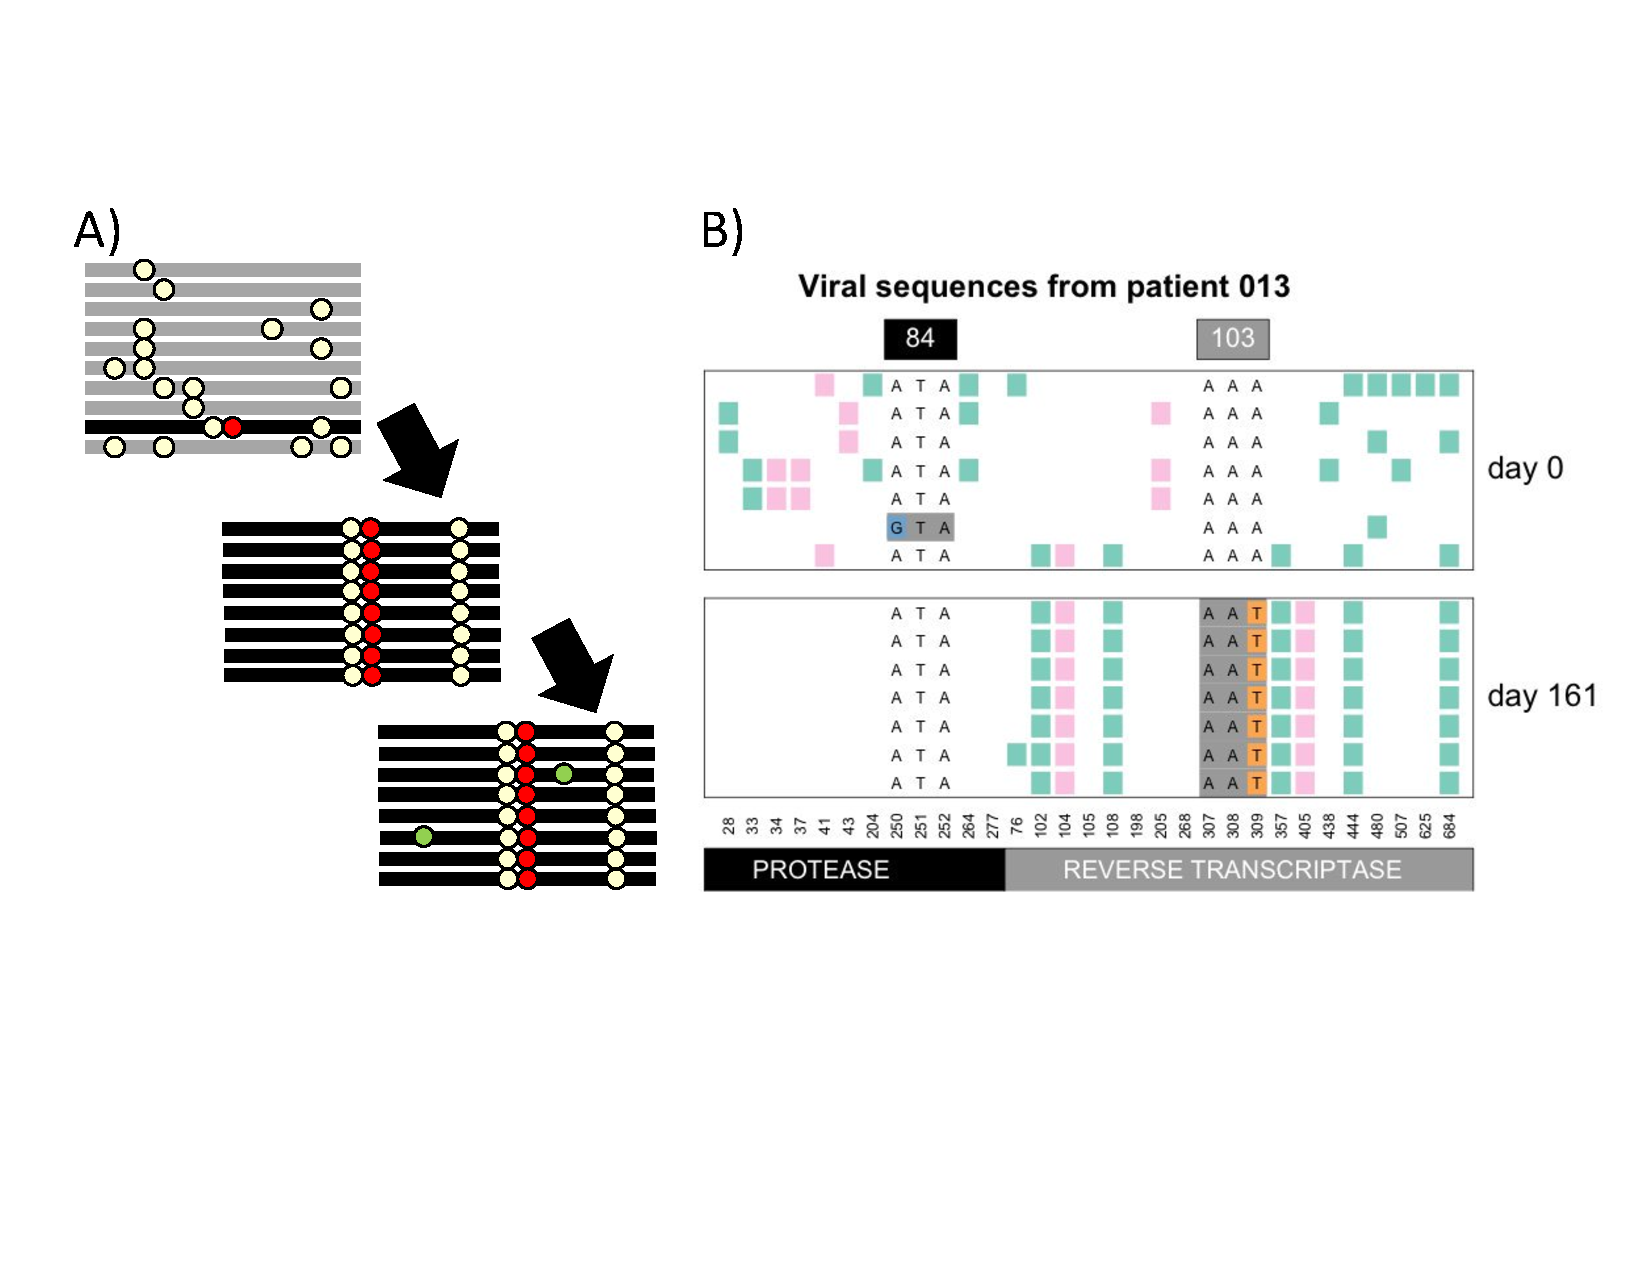
\includegraphics[width= \textwidth]{Journal_figs/recom_selection/Pleuni_HIV_sweep/HIV_no_recom_sweep.pdf}
\end{center}
\caption{{\bf A)} In the top panel a selected mutation (red dot) arises
on a particular haplotype in the population. It sweeps to fixation
carrying with it the haplotype on which it arose, middle panel,
erasing the standinggenetic diversity in the region. The bottom panel
is some time after the selective sweep when some new neutral alleles (green
dots) have started to drift up in frequency. {\bf B)}  Top panel: HIV
sequences from a patient at the start of drug treatment in the
protease and retrotransposase coding regions. Bottom panel: A sample
161 days later a drug resistant mutation has spread, the A
$\rightarrow$ T in the 103 codon of retrotransposase. Each row is a haplotype,
with the alleles present shown as coloured blocks. } \label{fig:HIV_sweep}
\end{figure}

Pleuni Pennings has been working on visualizing selective sweeps in
HIV. In Figure \ref{fig:HIV_sweep}B) we see a set of HIV haplotypes
sampled from a patient before and after of a selective sweep of a
drug-resistant mutation. The patient is taking a
retrotransposase inhibtator (Efavirenz), but sadly within 161 days a
drug-resistant mutation that changes the HIV retrotransposase ‏protein
has arisen and spread. Note how a particular haplotype is now fixed in
the sample, and little genetic diversity remains, due to the
hitchhiking effect of the strong
selective sweep of this allele. 


\begin{marginfigure}
\begin{center}
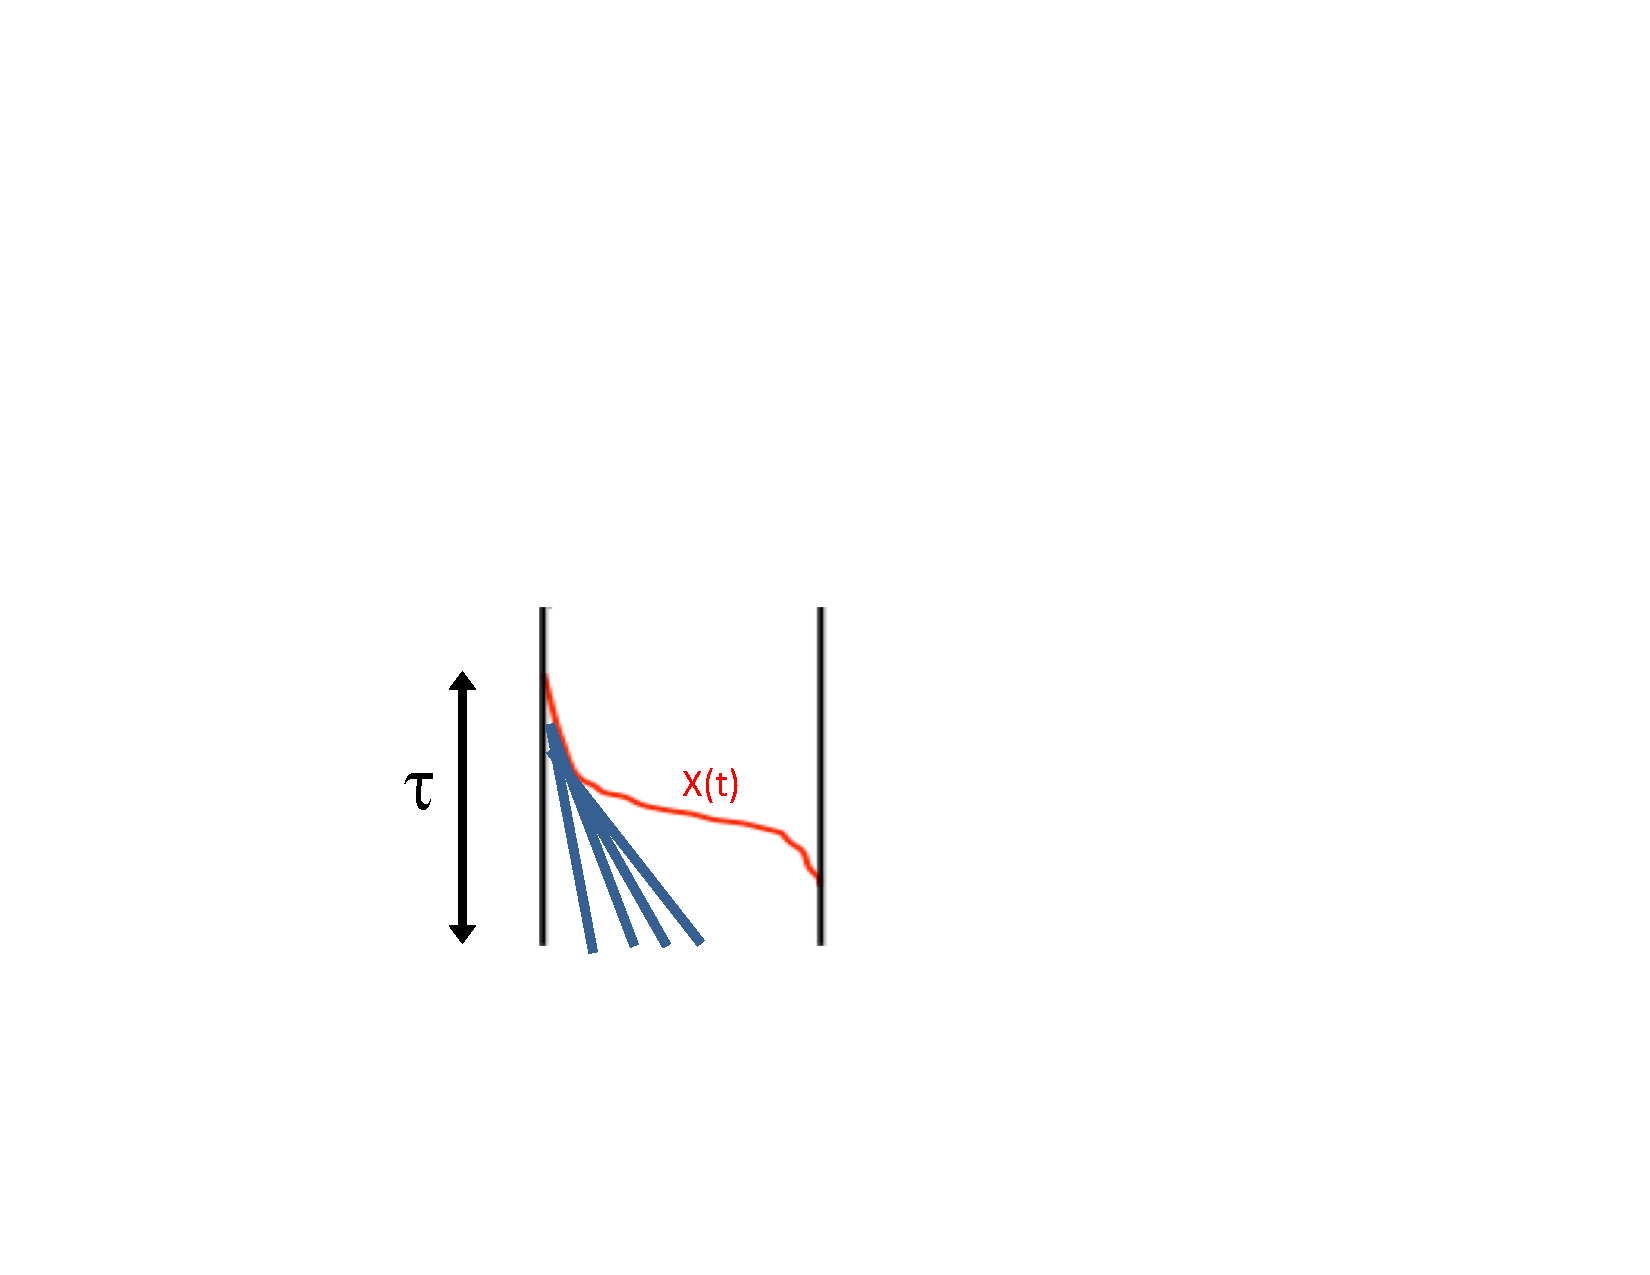
\includegraphics[width= 0.75 \textwidth]{figures/Hitchhiking/No_recom_coal.pdf}
\end{center}
\caption{} \label{fig:no_recom_coal}
\end{marginfigure}
First lets imagine examining variation at a locus fully linked
to our selected locus, just after our sweep reached fixation. Neutral alleles sampled at this locus
must h trace their ancestral lineages back to the neutral
allele on whose background the selected allele initially arose (Figure
\ref{fig:no_recom_coal}). As
that neutral allele, which existed $\tau$ generations ago is the
ancestor of the entire population at this locus. Our individuals who
carry the beneficial allele are, from the perspective of these two
alleles, exactly like a rapidly expanding population. Therefore, our
pair of neutral alleles sampled at our locus will be forced to
coalesce $\approx \tau$ generations ago. A newly derived allele with an additive selection coefficient $s$ will
take a time $\tau \propto \log(N)/s$ generations to reach to fixation
within our population (see eqn. \eqref{eq:diploid_fix_time}). This is a very
short-time scale compared to the average neutral coalescent time of
$2N$ generations of a pair of alleles. Thus we expect little variation
as few mutations will have arisen on these very short branches, and
those that have done will likely be singletons in our sample. \\

\begin{marginfigure}
\begin{center}
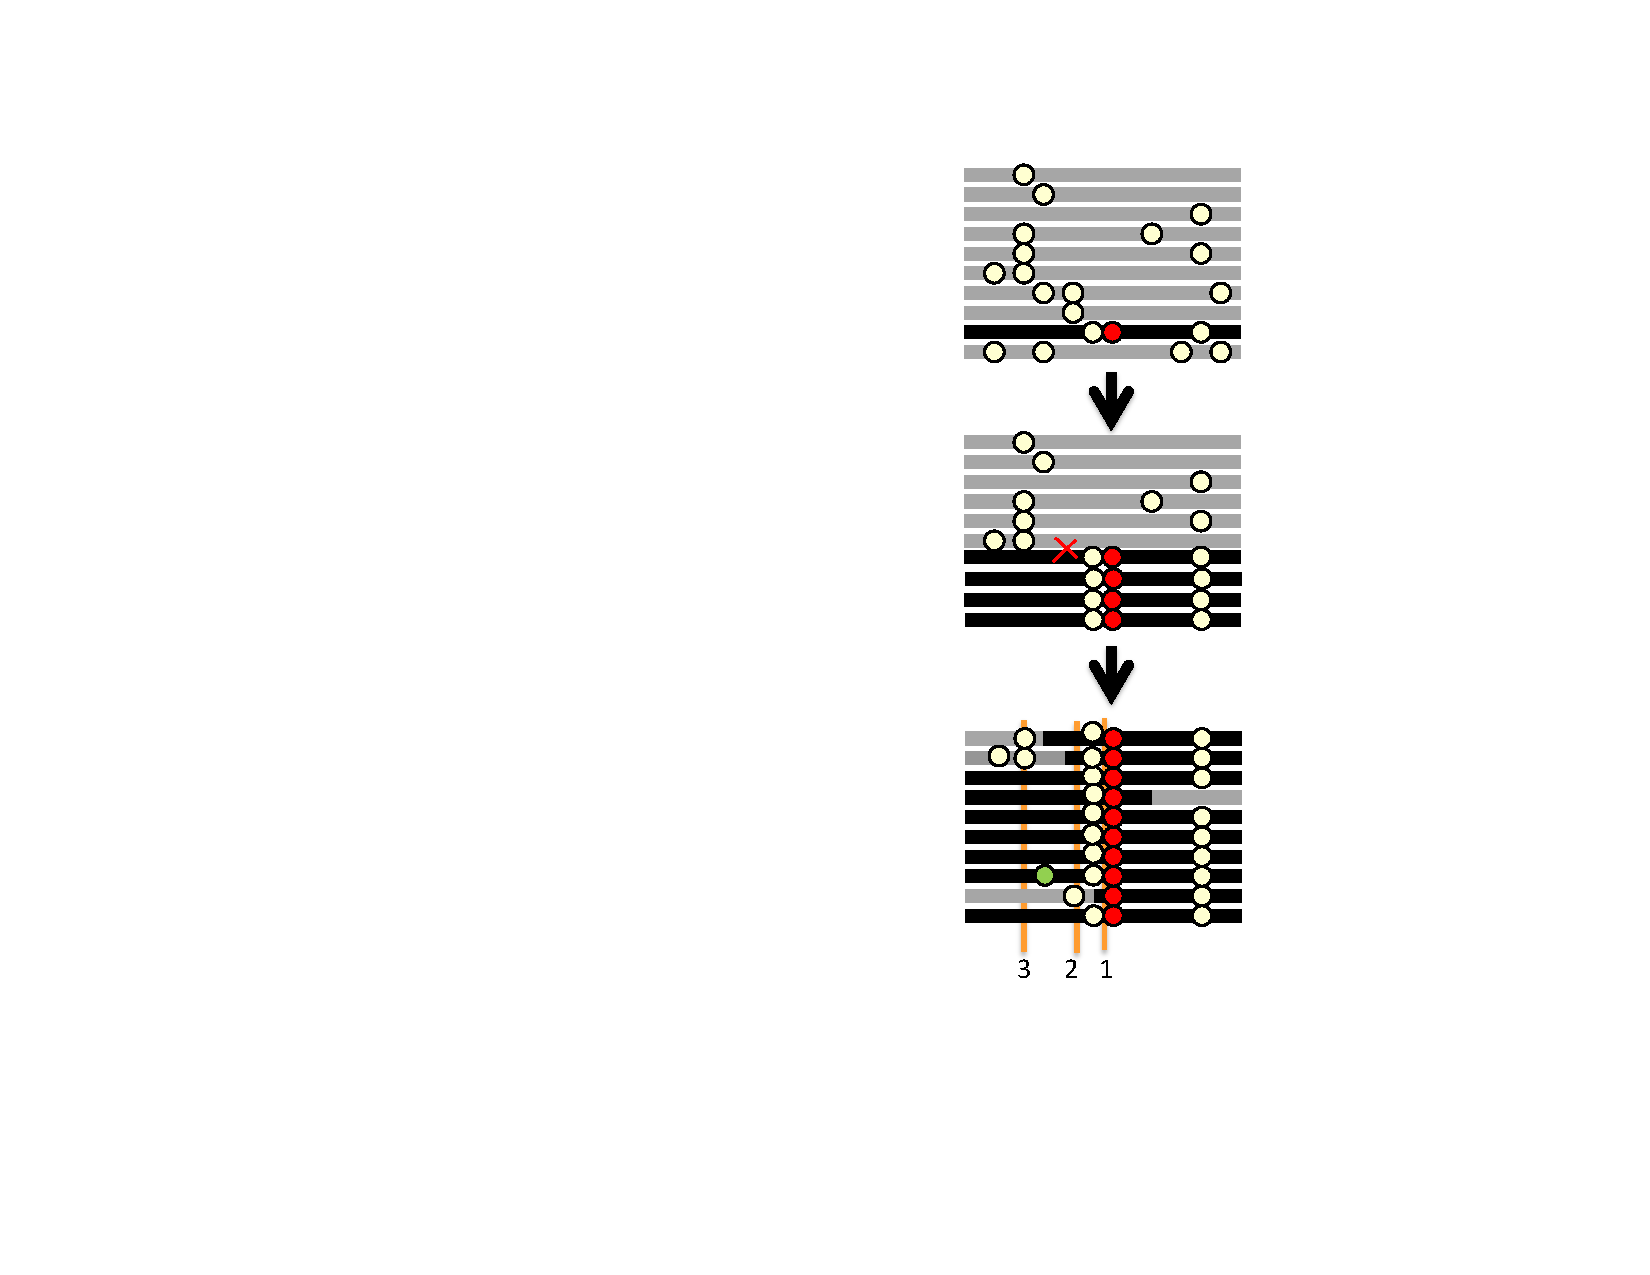
\includegraphics[width= 0.5 \textwidth]{figures/Hitchhiking/recom_haps_sweep.pdf}
\end{center}
\caption{} \label{fig:sweep_haps}
\end{marginfigure}
Now let's think about a sweep in a recombining region. Again the
selected mutation arises on a particular haplotype, and it and its
haplotype starts to increase in frequency in the population. However,
now recombination events can occur between haplotypes carrying and not
carrying the selected allele, in individuals who are heterozygote for
the selected allele. These recombination events allow alleles that
were not present on the original selected haplotype to avoid being
swept out of the population, and also decouple the selected allele
somewhat from hitchhiking alleles preventing them from hitchhiking all
the way to fixation. Far out from the selected site the recombination
rate isd high enough that alleles that were present on the original
background barely get to hitchike along as recombination breaks up
their association with the selected allele very rapidly.

\begin{figure}
\begin{center}
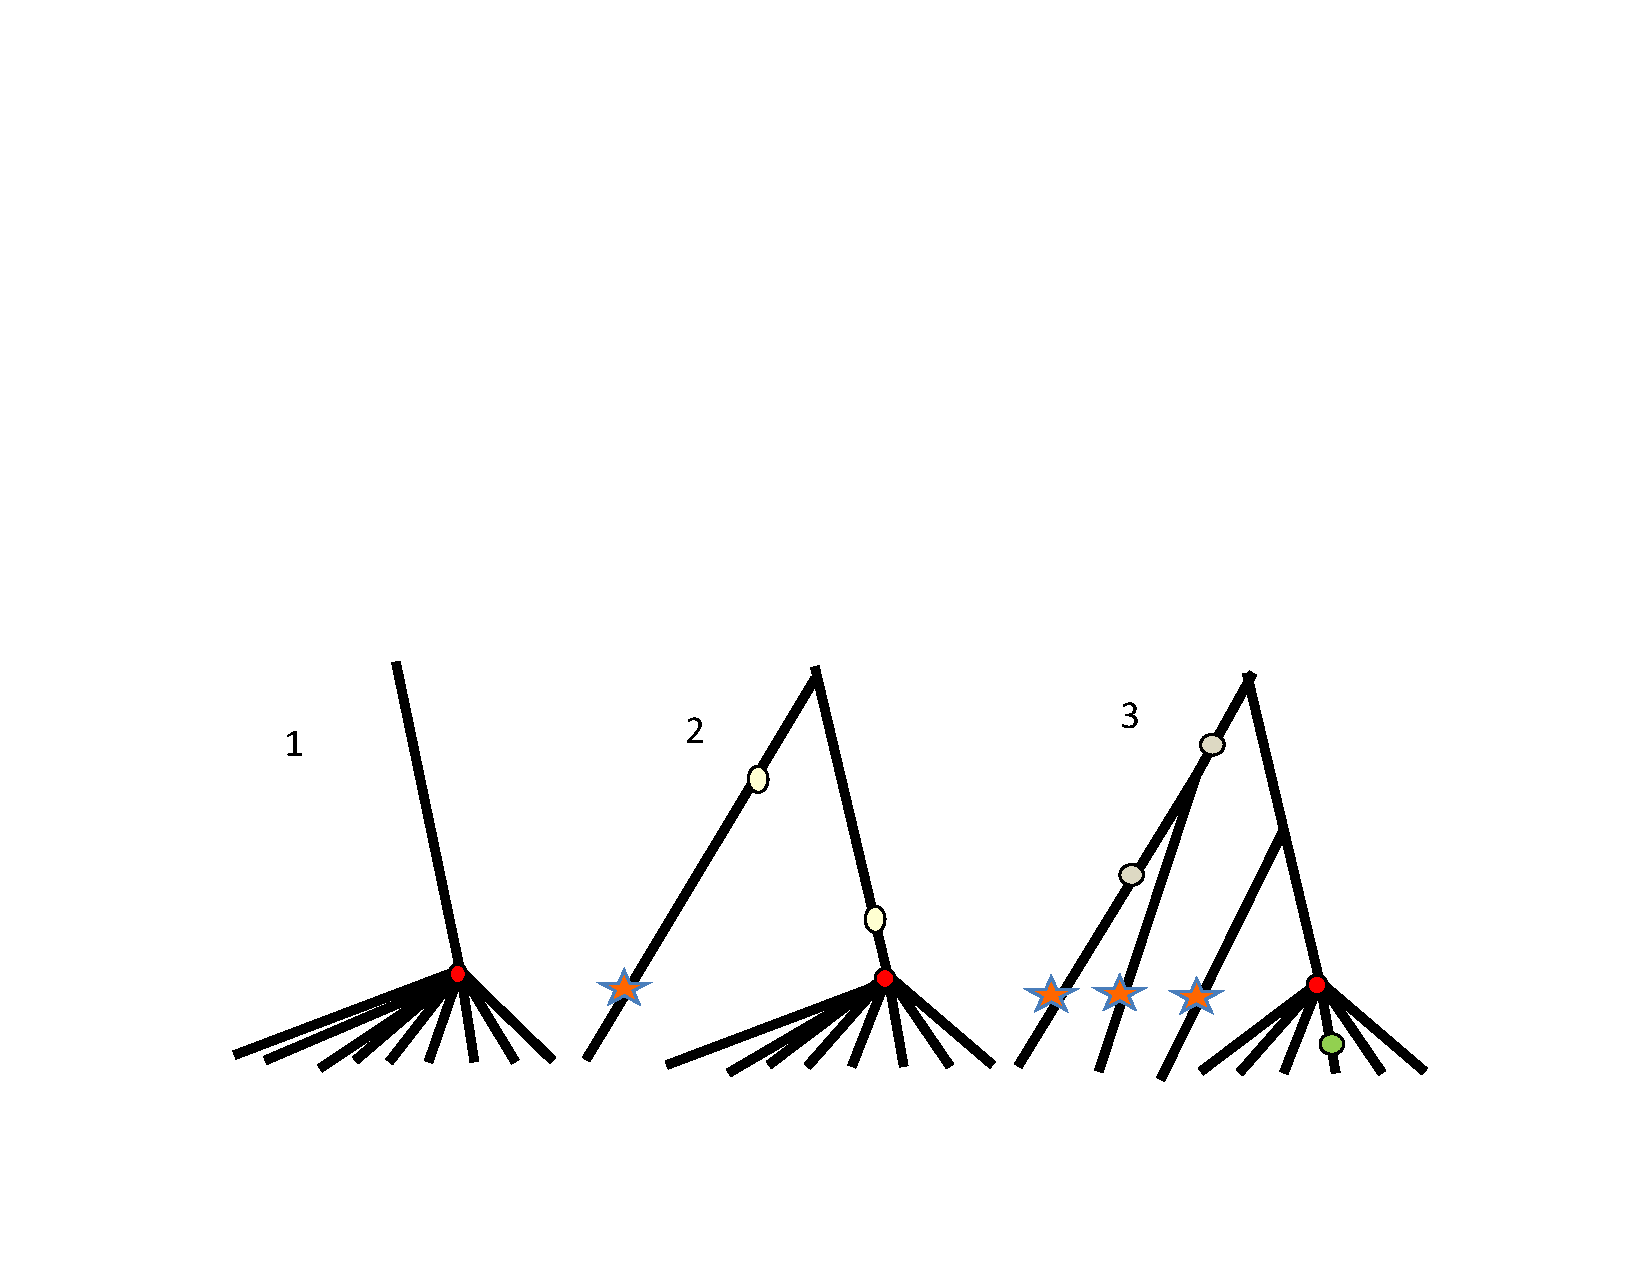
\includegraphics[width= 0.9 \textwidth]{figures/Hitchhiking/recom_haps_coal_sweep.pdf}
\end{center}
\caption{} \label{fig:sweep_haps_coal}
\end{figure}

What do the coalesecent genealogies look like at loci various distances away from the
selected site? Well close to the selected site all our alleles in the
present day trace back to a most recent common ancestral allele
present on that selected haplotype, and so are all forced to coalesce
around $\tau$ generations ago (locus 1). Slightly further out from the selected
site (locus 2), we have lineages that don't trace their ancestry back
to the original selected haplotype, but instead are descended from
recombinant haplotypes that recombined onto the sweep (the haplotype 2 from the
bottom). These lineages can coalesce neutrally with the other ancestral lineages
over far deeper time scales, mutations on these deeper lineages
corresponding to the standing diversity present in our population
prior to the sweep. As we move even further out from the selected site
(locus 3) we encounter more an more lineages descended from
recombinant haplotypes that coalescent neutrally much deeper in time
allowing diversity to recover to background levels as we move away
from the selected site.

\begin{figure}
\begin{center}
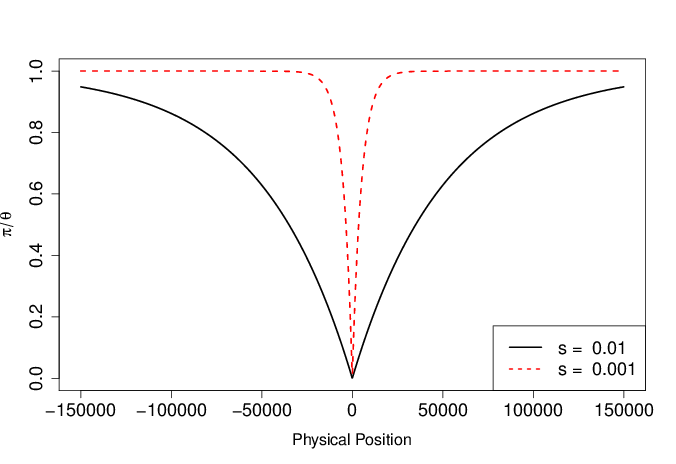
\includegraphics[width=0.75\textwidth]{figures/hitchhiking_reduction.png}
\end{center}
\caption{Reduction in diversity compared to its neutral expectation as
a function of the distance away from a site where a selected allele
has just gone to fixation. The recombination rate is $r_{BP}= 1\times
10^{-8}$.} \label{fig:hitchhiking_reduction}
\end{figure}



\begin{marginfigure}
\begin{center}
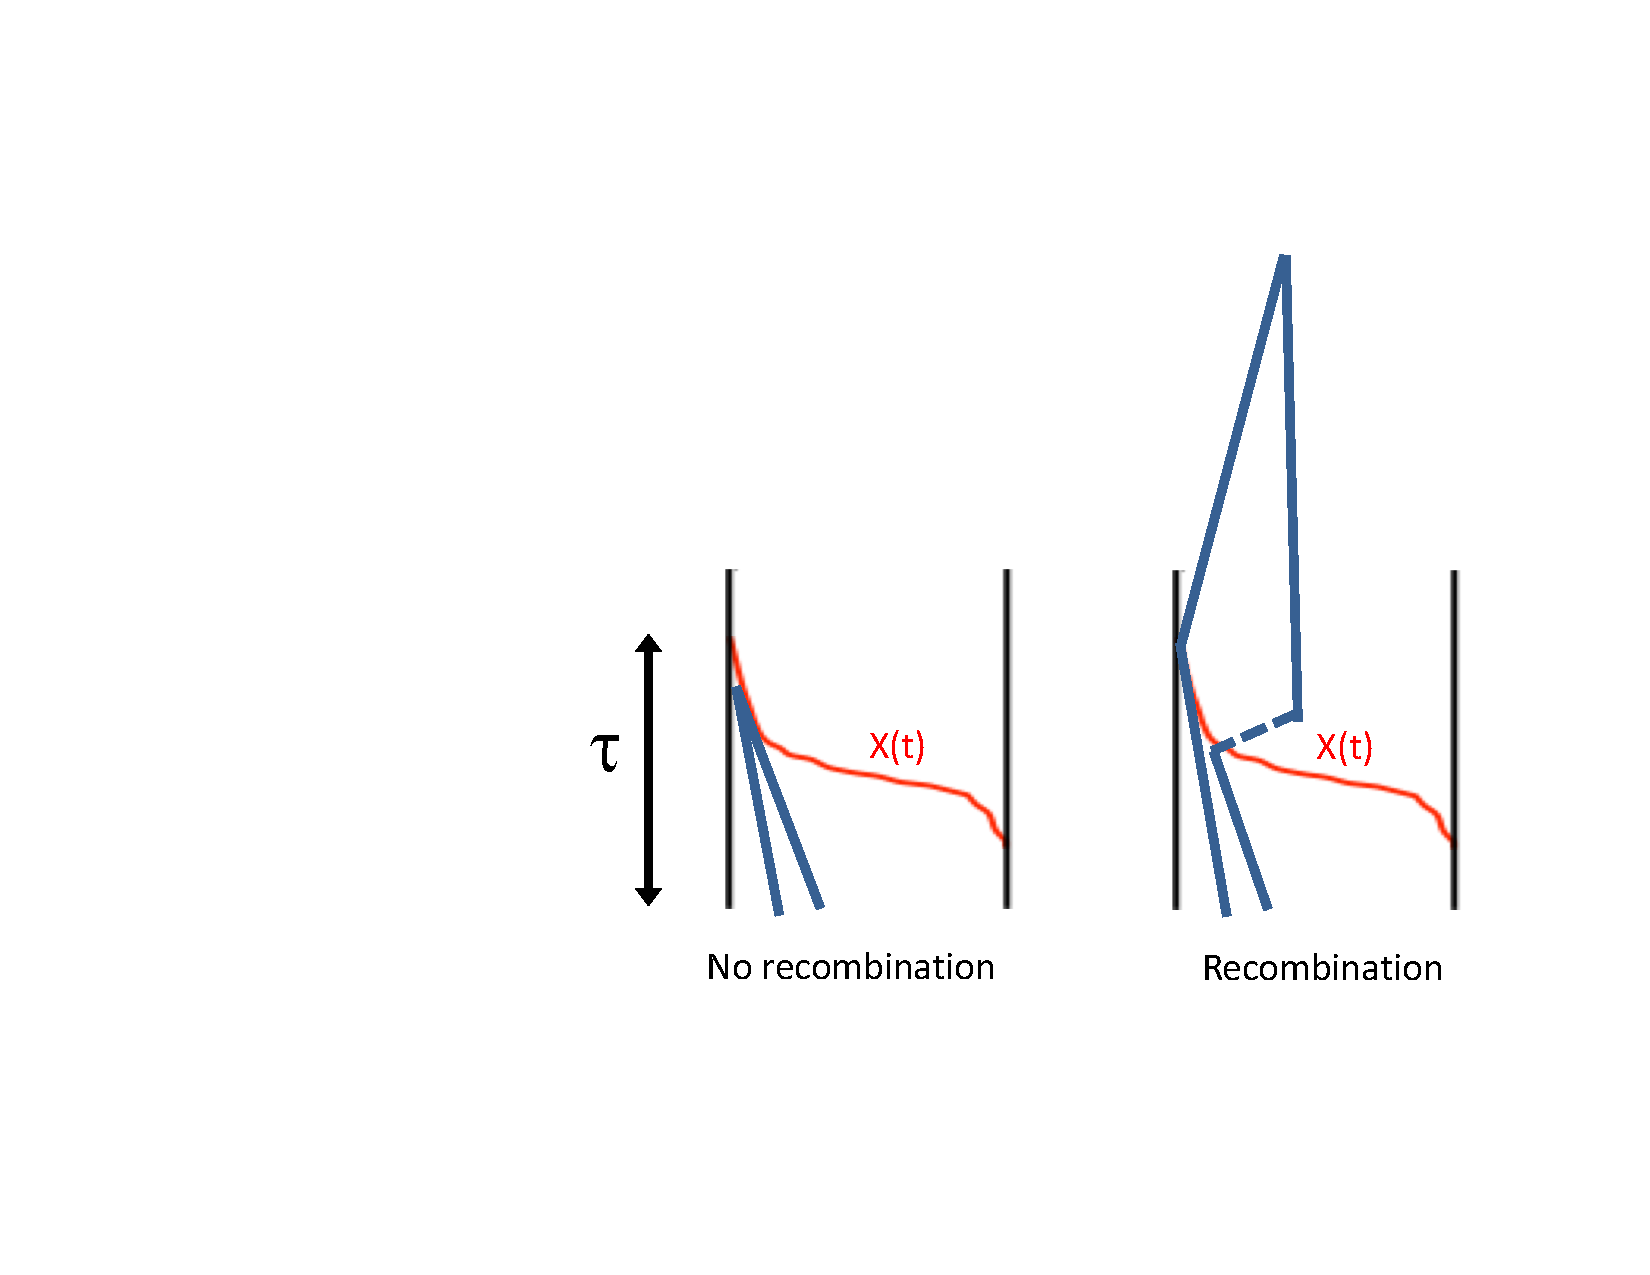
\includegraphics[width= \textwidth]{figures/Hitchhiking/Recom_coal.pdf}
\end{center}
\caption{} \label{fig:no_recom_coal}
\end{marginfigure}
To model the expected pattern of diversity surrouding a selected site we can think about a pair
of alleles sampled at a neutral locus a recombination distance $r$
away from our selected site. Our pair of alleles will be forced to
coalesce $\approx \tau$ generations if neither of them of are
descended from recombinant haplotypes.\\

We know that in the present day that our neutral lineage is linked to
the selected allele. The probability that our lineage, in some
generation $t$ back in time, is in a heterozygote is $1-X(t)$, the
probability that a recombination occurs in that indvidual is $r$. So
the probability that our neutral lineage is descended from a
recombinant haplotype $t$ generations back is 
\begin{equation}
r (1-X(t))
\end{equation}
so the probability ($p_{NR}$) that our lineage is not descended from a
recombinant haplotype in the
$\tau$ generations it takes our selected allele to move through the
population is
\begin{equation}
p_{NR}=\prod_{t=1}^{\tau} \big(1- r(1-X(j))\big)
\end{equation}
assuming that $r$ is small then $ \left(1- r(1-X(t))\right) \approx
e^{-r(1-X(t))}$, such that
\begin{equation}
p_{NR}=\prod_{t=1}^{\tau} \left(1- r(1-X(t))\right) \approx \exp
\left( -r\sum_{t=1}^{\tau}
1- X(t) \right) =\exp
\left( -r \tau (1-\widehat{X}) \right)
\end{equation}
where
$\widehat{X}$ is the average frequency of the derived allele across the trajectory
$\widehat{X} = \frac{1}{\tau}  \sum_{t=1}^{\tau}
 X(t)$. As our allele is additive its trajectory for frequencies
 $<0.5$ is the mirror image of its trajectory for frequency $>0.5$, therefore it
average frequency $\widehat{X} =0.5$. So
\begin{equation}
p_{NR} = e^{-r \tau/2 }.
\end{equation}
The probability that neither of our lineages is descended from a
recombinant haplotype and hence are forced to coalesce is $p_{NR}^2$, assuming that
they coalesce at a time close to $\tau$ so that they recombine
independently of each other for times $< \tau$.\\

If one or other of our lineages is descended from a recombinant haplotype it will take them on average
$\approx 2N$ generations to find a common ancestor as we are back our
neutral coalescent. Thus the expected time
till our pair of lineages find a common ancestor is
\begin{equation}
\E(T_2)  = \tau \times p_{NR}^2 +(1-p_{NR}^2) (\tau +2N) \approx
\left(1-p_{NR}^2 \right) 2N
\end{equation}
where this last approximation assumes that $\tau \ll 2N$. So the
expected pairwise diversity for neutral alleles at a recombination
distance $r$ away from the selected sweep  ($\pi_r$) is
\begin{equation}
\E(\pi_r) = 2\mu \E(T_2)  \approx \pi_0 \left(1-e^{-r\tau} \right) \label{eqn:pi_HH}
\end{equation}
so diversity increases as we move away from the selected site,
slowly exponentially plauteuing to its neutral expectation $\pi_0$.\\

The malaria pathogen ({\it Plasmodium falciparum}) has
evolved drug resistance to anti-malaria drugs, often by changes at
their dhfr gene. Figure \ref{fig:hitchhiking_malaria} shows levels of
genetic diversity (heterozygosity) at a set of markers moving out from the dhfr gene in a
set of  drug resistant malaria sequences collected in
Thailand \citep{nash2005selection}. We see the characteristic dip in diversity around the gene,
with zero diversity at a number of the loci very close to the gene,
suggesting a strong selective sweep. Fitting our simple model of a
sweep to this data,  we estimate that $\tau \approx 40$ generations
corresponding to the drug-resistance allele fixing in very short time period. 
% these drug (Sulfadoxine–pyrimethamine) 

\begin{figure}
\begin{center}
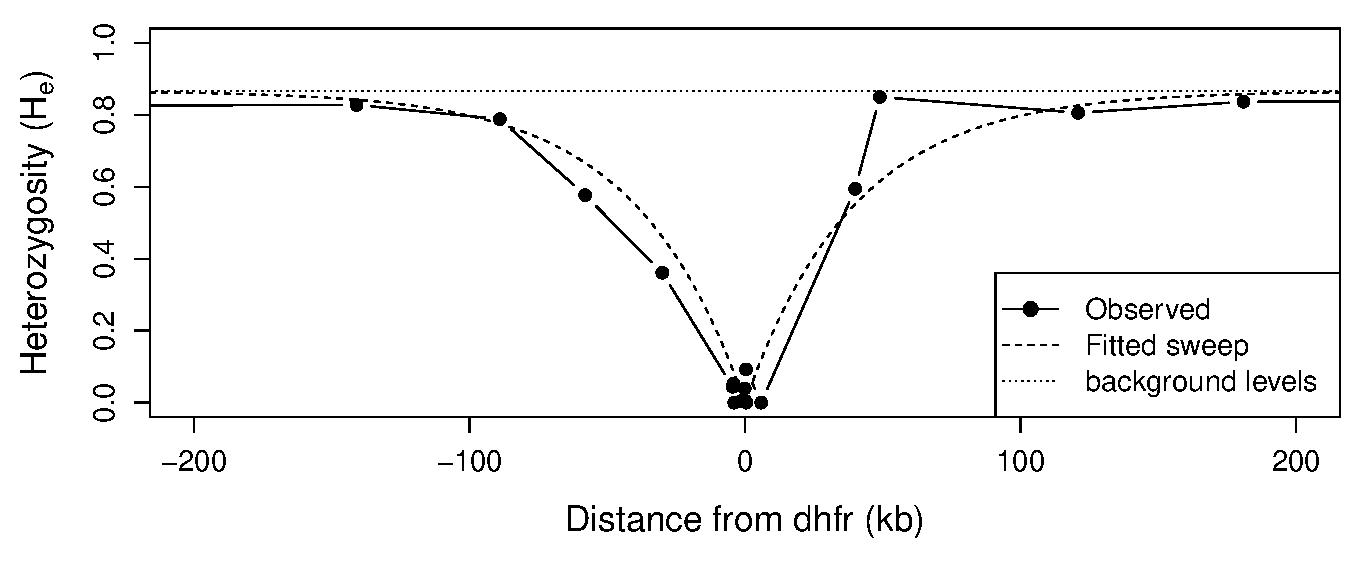
\includegraphics[width=\textwidth]{Journal_figs/recom_selection/malaria_sweep/dhfr_sweep.pdf}
\end{center}
\caption{Levels of heterozygosity at a set of microsatellite markers
  surounding the dhfr gene in samples of drug-resistant malaria ({\it Plasmodium falciparum}) from
  Thailand. The dotted horizontal line gives the average level of
  heterozygosity found at these markers in a set of drug-resistant
  malaria, we take this background as our $\pi_0$. Data from \citet{nash2005selection}. The dash line shows
  our fitted hitchhiking model from equation \ref{eqn:pi_HH} with $\tau \approx 40$, fitted by
  non-linear least squares. } \label{fig:hitchhiking_malaria}
\end{figure}


To get a sense of the physical scale over which diversity is reduced
consider a region where recombination occurs at a rate $r_{BP}$ per
base pair per generation, and our locus is $ \ell $ base pairs away from the
selected site $r=r_{BP } \ell $ (where $r_{BP}  \ell  \ll 1$ so we don't need to
worry about more than one recombination event occurring per
generation). Typical
recombination rates are on the order of $r_{BP} = 10^{-8}$, in Figure
\ref{fig:hitchhiking_reduction} we show the reduction in diversity,
given by eqn. \eqref{eqn:pi_HH}, for two different selection coefficients.\\ 

For our expected diversity levels to recover to $50\%$ of
its neutral expectation $\E(\pi_r)/\theta=0.5$, requires a physical
distance $\ell^{*}$ such that $\log(0.5) = -r_{BP} \ell ^*\tau$ as using our
expression for $\tau$ then $ \ell^* = \frac{-\log(0.5)}{r_{BP} \tau }$. As
$\tau$ depends inversely on the selection $s$ (eqn. \eqref{eq:diploid_fix_time}), the width of our trough of reduced diversity depends on $s/r_{BP}$.
All else being equal we expect stronger sweeps or sweeps in regions of low
recombination to have a larger hitchhiking effect. So that a selection coefficient of $s=0.1\%$ would reduce
diversity over 10's of kb, while a sweep of $s=1\%$ would affect
$\sim$100kb.   \\


\begin{question}
A recently published study has identified the genetic basis of
melanism in the pepper moth. This allele swept to fixation in northern
parts of the UK; a classic case of adaptation to industrial pollution
(made famous by the work of Kettlewell). The genetic basis of melanism
is a transposable element (TE) inserted into a pigmentation gene. The
investigators found that diversity is suppressed in a broad region
around the TE. Specifically, on the background of the TE, it takes
roughly 200 kb in either direction for diversity levels to recover to
50\% of genome-wide levels. \\

Random facts: In all moths and butterflies only males recombine;
chromosomes are transmitted without recombination in female. The
recombination rate in males is 2.9 cM/Mb.  Peppered moths have an
effective population size of roughly a hundred thousand
individuals. Kettlewell used to eat moths when out collecting them in
the field (personal communication, Art. Shapiro). \\
{\bf A)} Briefly explain how this pattern offers further evidence that the melanic allele was favoured by selection.\\
{\bf B)} Using this information what is your estimate as to the age of the allele?\\
{\bf C)} What is your estimate of the selection coefficient favouring this melanic?
\end{question}


\subsection{A simple recurrent model of selective sweeps}
We sample a pair of neutral alleles at a locus a genetic distance $r$ away from a locus where
sweeps are initiated within the population at some very low rate $\nu$
per generation. The waiting time between sweeps
at our locus is exponential $\sim Exp(\nu)$. Each sweep rapidly transits through the population in $\tau$
generations, such that each sweep is finished long before the next
sweep ($\tau \ll 1/\nu$). \\

As before our chance that our neutral lineage fails to recombine
off the sweep is $p_{NR}$, such that the probability that
our pair of lineages are forced to coalesce by a sweep $e^{-r \tau}$. Our
lineages therefore have a very low probability
\begin{equation}
\nu e^{-r \tau}
\end{equation}
of being forced to coalesce by a sweep per generation. In addition of
lineages can coalesce at a neutral rate of $1/(2N)$. Thus the average
waiting time till a coalescent event between our neutral pair of
lineages due to either a sweep or a neutral coalescent event is
\begin{equation}
\E(T_2) = \frac{1}{\nu e^{-r \tau} + 1/(2N)}
\end{equation}

Now imagine that the sweeps don't occur at a fixed location with
respect to our locus of interest, but now occur uniformly at random
across our sequence. The sweeps are initiated at a very low rate of
$\nu_{BP}$ per basepair per generation. The rate of coalescent due to
sweeps at a locus $\ell$ basepairs away from our neutral loci is
$\nu_{BP} e^{-r_{BP} \ell \tau}$. If our neutral locus is in the
middle of a chromosome that stretches $L$ basepairs in either direction
the total rate of sweeps per generation that force our pair of lineages to coalesce is
\begin{equation}
2\int_0^{L} \nu_{BP} e^{-r_{BP} \ell \tau} d \ell =
\frac{2\nu_{BP}}{r_{BP} \tau} \left(1-e^{-r_{BP} \tau L} \right)
\end{equation}
so that if $L$ is very large ($r_{BP} \tau L \gg 1$) the rate of coalesce per
generation due to sweeps is $\frac{2\nu_{BP}}{r_{BP} \tau}$. The total rate
of coalescence for a pair of lineages per generation is then
\begin{equation}
\frac{2\nu_{BP}}{r_{BP} \tau}+\frac{1}{2N}
\end{equation}
So our average time till a pair of lineages coalesce is
\begin{equation}
\E(T_2) = \frac{1}{\frac{2\nu_{BP}}{r_{BP} \tau}+\frac{1}{2N}} = \frac{r_{BP}2N}{\frac{4N\nu_{BP}}{ \tau}+r_{BP}}
\end{equation}
such that our expected pairwise diversity ($\pi=2\mu\E(T_2)$) in a region of
recombination rate $r_{BP}$ that experiences sweeps at rate $\nu_{BP}$
is  
\begin{equation}
\E(\pi) = \theta \frac{r_{BP}}{\frac{4N\nu_{BP}}{ \tau}+r_{BP}} \label{eqn:pi_GW_HH}
\end{equation}


\begin{figure}
\begin{center}
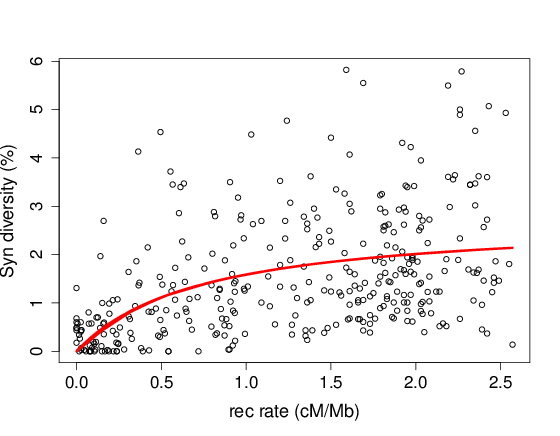
\includegraphics[width=0.5\textwidth]{figures/Genomewide_HH.png}
\end{center}
\caption{The relationship between (sex-averaged) recombination rate and synonymous
  site pairwise diversity ($\pi$) in {\it Drosophila melanogaster}
  using the data of Shapiro et al. 07 (kindly provided by Peter
  Andolfatto, see Sella et al. 09 for details). The curve is the
  predicted relationship between $\pi$ and recombination rate obtained
  by fitting equation \eqref{eqn:pi_GW_HH} to this data 
 using non-linear least squares via the {\tt nls()} function in {\tt R}.} \label{fig:GW_hitchhiking_reduction}
\end{figure}



